\documentclass[border=10pt]{standalone}
\usepackage{pgfplots}
\pgfplotsset{compat=1.17}

\begin{document}
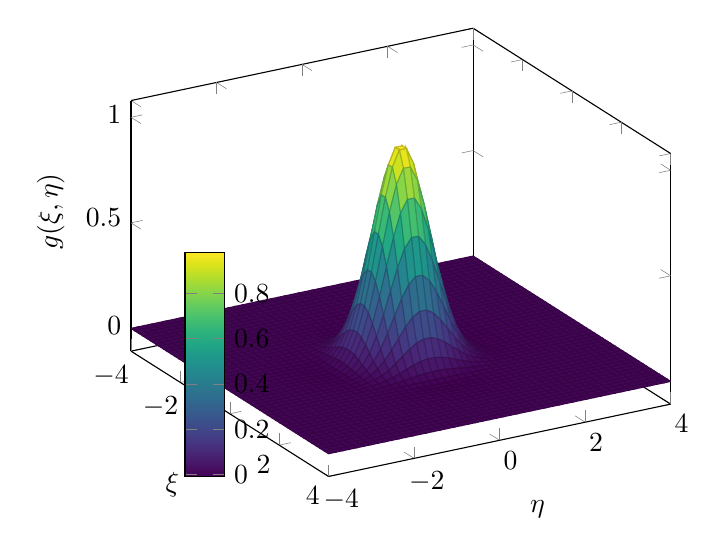
\begin{tikzpicture}
    \begin{axis}[
        xlabel=$\xi$,
        ylabel=$\eta$,
        zlabel={$g(\xi, \eta)$},
        view={60}{30},
        domain=-4:4,
        y domain=-4:4,
        samples=50,
        colormap/viridis,
        colorbar,
        colorbar style={
            at={(0.1,0)},
            anchor=south west,
            height=0.5*\pgfkeysvalueof{/pgfplots/parent axis height},
            title={}
        }
    ]
        \addplot3[surf] {exp(-x^2-y^2)*cos(deg(x))*cos(deg(y))};
    \end{axis}
\end{tikzpicture}
\end{document}